\label{sec:results}

The final stage of our analysis involves applying the two-level aggregation model to the decision matrix to rank the 29 alternative schedules. The model's flexibility allows a decision-maker to articulate their preferences through two sets of parameters: a preference for seasonality (3 weights) and an overall attitude towards risk, defined by the orness value $\alpha$. To showcase the model's behavior, we present the results across a spectrum of these parameters. Figure \ref{fig:results_plot} visualizes the outcomes for four distinct seasonal scenarios: a singular focus on each of the three seasons, and an equal weighting for all. 

The weight vectors for (Winter, Summer, Inter-season) used in these scenarios are (1.0, 0.0, 0.0) for ``Winter focus", (0.0, 1.0, 0.0) for ``Summer focus", (0.0, 0.0, 1.0) for ``Inter-season", and (1/3, 1/3, 1/3) for ``Equal weights"

\begin{figure}[h!]
    \centering
    \begin{adjustwidth}{-1.2cm}{-1.8cm}
    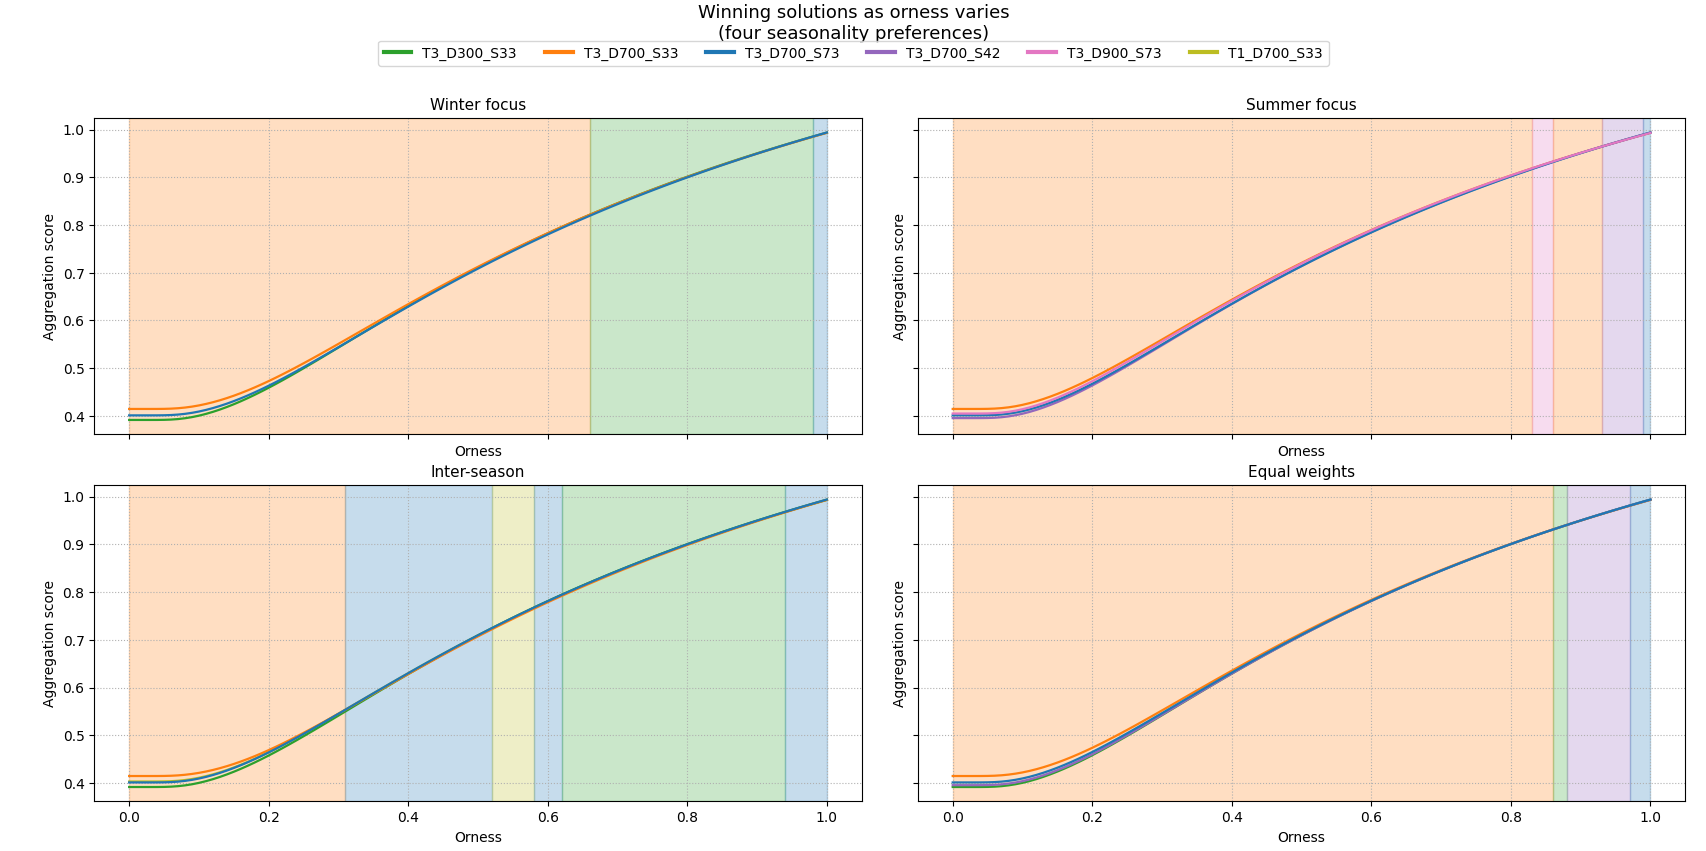
\includegraphics[width=1.08\textwidth]{ch3/figures/ResultsOrness.png}
    \end{adjustwidth}
    \caption{Final aggregation scores for the top-performing solutions across the full range of orness values ($\alpha$). Each subplot corresponds to a different seasonal preference. The colored vertical bands highlight the range of orness values for which a particular solution (identified in the legend) is optimal.}
    \label{fig:results_plot}
\end{figure}

The orness parameter, $\alpha$, critically shapes the final ranking by controlling the OWA operator's behavior. As $\alpha$ approaches 0, the aggregation mirrors a \textit{min} operator, reflecting a pessimistic or risk-averse attitude. In this regime, the decision is driven by the worst-performing attribute for each alternative. Given that the `Highest Concurrency` scores (around 0.4) are numerically much lower than the fuzzy attribute scores (all above 0.9) or seasonality (around 0.6), it becomes the dominant criterion. Consequently, for low orness values, the model consistently selects solution \texttt{T3\_D700\_S33}, as it features the most favorable (i.e., lowest) highest concurrency.\\

Conversely, as $\alpha$ approaches 1, the OWA operator emulates a \textit{max} operator, reflecting an optimistic stance that judges an alternative by its strongest attribute. In this scenario, the model favors solutions that excel in at least one key area. The results show that for high orness values, solution \texttt{T3\_D700\_S73} is predominantly chosen because it achieves the highest score in ``Risk Concurrency", which represents the most uniform distribution of high-risk interventions.\\

Across the four seasonal scenarios and the entire orness spectrum, a total of seven distinct solutions emerged as optimal at some point. It is noteworthy that six of these seven top-performing solutions were generated by the algorithm from Team 3, signaling its ability to produce robust and high-quality schedules. The exception, solution \texttt{T1\_D900\_S33} from Team 1, becomes the preferred choice under the ``Inter-season focus" scenario for orness values slightly above 0.5, corresponding to a moderately optimistic viewpoint. Furthermore, our epsilon-lexicographic method for handling intra-block aggregation proved effective: across 23 instances where ties occurred based on the primary criterion, the rankings were successfully resolved through consideration of the second most relevant attribute in the hierarchical structure.\\

Another relevant aspect shown in Figure \ref{fig:results_plot} is the tiny differences in the aggregated score of different solutions. This observation is further supported by the decision matrix (table \ref{tab:dm_matrix}), which reveals remarkably small variance within each column. While the heatmap (Figure \ref{fig:dif_sol}) shows that schedules can differ by hundreds of intervention start times, the attribute scores remain highly similar across solutions. This apparent contradiction is explained by how the criteria are defined and the problem's inherent constraints. The attributes are primarily dependent on the overall (shape) distribution of interventions, as all solutions must organize the exact same interventions. The highly constraints of the original problem led algorithms to naturally converge towards solutions that share a common strategy for overall workload distribution, even if they differ in specific intervention timings. Therefore, our attributes are too general and lack discriminative power, and more specific criteria focused on particular days or interventions might provide better differentiation. However, such approaches would require more detailed information than what is publicly available. The decision matrix thus captures only subtle variation of the alternatives on a common optimized approach rather than fundamentally different scheduling paradigms. \\

Due to these limitations, several avenues for future research can be suggested. A more powerful analysis could be conducted by incorporating more granular, non-public data. For instance, information on the specific economic impact of delaying certain power lines, the criticality of interventions in different geographical zones, or scenario-specific risk profiles could be used to develop more targeted criteria. Future work could also focus on designing attributes that move beyond general uniformity, such as criteria that explicitly penalize interventions during historically critical periods (e.g., Christmas days) or measure the temporal clustering of specific intervention types. Nevertheless, even with its current limitations, the proposed framework successfully provides a transparent and intuitive method for navigating these complex decisions, offering a justifiable basis for selecting a final schedule from a pool of highly competitive options.